\documentclass{llncs}

\usepackage{llncsdoc}
\usepackage{graphicx,url}
\usepackage[USenglish]{babel}
\usepackage[utf8]{inputenc}
\usepackage{float}
\usepackage{setspace}

\usepackage{tabularx}
\usepackage{cite}
\usepackage{hyperref}
\usepackage{subcaption}

\begin{document}
\sloppy
\title{Mezuro: Understading source code metrics} % só remover o understanding?

\author{Dylan Guedes\inst{1}, Paulo Meirelles\inst{1,2},
        Rafael Manzo\inst{2}, Diego Camarinha\inst{2}}


\institute{Faculdade do Gama -- Universidade de Brasília (UnB)\\
  Área Especial de Indústria Projeção A -- Setor Leste -- Gama -- DF -- Brazil \\
  \email{120115727@aluno.unb.br,paulormm@unb.br}
  \and
  Instituto de Matemática e Estatística -- Universidade de São Paulo (USP)\\
  Rua do Matão, 1010 -- 05508-090 -- Cidade Universitária -- São Paulo -- SP -- Brasil\\
  \email{\{paulormm,manzo,diegoamc\}@ime.usp.br}}

\maketitle
\begin{abstract}
  % Contexto
  The ease of development and maintenance of a software is directly related
with its quality.
  % Problema
  However, its source code analysis has issues, such as, the definition of
which metrics to use and how to interpret the results. Furthermore, this
practice is still not common on industry development workflow. Those who % não removi o _on_
decide to employ source code analysis lack free software alternatives that
integrate multiple languages and tools.
% Soluções propostas
  In this work we present Mezuro: a FOSS web-based platform to collaboratively
analyze source code. The project provides ways to compare projects and share
knowledge about metrics, teaching how to configure and interpret them. The
platform was planned to integrate multiple metric collectors for several
programming languages, and, currently, allows analysis of source code written
in C, C++, Java, Ruby, PHP, and Python.
  % Frase de impacto
  With this project we aim to spread knowledge and encourage the use of % expect por aim?
code metrics by the free software developer community.

\textbf{Keywords:} static analysis, source code metrics, open source software.
\end{abstract}

\section{Introduction}
\label{sec:intro}

Static source code metrics are measures extracted from the code without
compiling or running it. For example, these metrics provide information about
complexity, comprehension, testability, maintainability, and evolution of code,
supporting software engineers to observe and determine source code
quality\cite{mills1988}.

Nowadays, several tools are used to extract source code metrics, such as
pylint\footnote{\url{pylint.org}} (Python),
metric\_fu\footnote{\url{github.com/metricfu/metric_fu}} (Ruby), and
Analizo (C/C++ and Java)\cite{terceiro2010analizo}, each one with different
levels of usability, definitions and set of metrics, being necessary the
creation of a platform that brings and present these results to the end user,
specially in tracking the software quality during its life cycle. Code metric
tools, in general, do not present a friendly interface, and, even more, do not
follow a standard.

Therefore, this work present the Mezuro platform, which (i) provides a single
interface grouping available tools;
(ii) allows selection and composition of metrics in a flexible manner;
(iii) preserves the evolution history;
(iv) presents results in a friendly way;
(v) allows users to customize the given interpretation accordingly to their own context.

\section{Related tools}

There are two tools related to Mezuro. The first,
SonarQube\footnote{\url{sonarqube.org}}, is a FOSS software
licensed as LGPLv3, and offers a platform to manage software quality by using
plugins through a
library\footnote{\url{docs.sonarqube.org/display/PLUG/Plugin+Library}}.
At its most basic version it classifies code problems and evaluate simple
coverage metrics in several languages. However, its best plugins are paid and
closed source, such as the C/C++
analyzer\footnote{\url{sonarsource.com/why-us/products/codeanalyzers/sonarcfamilyforcpp.html}}.

The second, Code Climate\footnote{\url{codeclimate.com}} is a tool
that analysis source code hosted in a Git server, and has support for several
programming languages and frameworks. The analysis will look for code smells
in the code and classify them based on aspects such as size of methods and
code duplication. Lastly, based on the score of its parts, the given project % mantive o lastly
will receive a grade ranging from A to F. Keep in mind that what is tagged as an
issue sometimes might not be a real problem, since it could be the best solution for % não troquei _issue_ por _smell_, avaliar
the given scenario. Such as SonarQube, Code Climate is FOSS, but without its
polished front-end, which makes Mezuro still the only complete FOSS alternative.
% pra mim ficou que o codeclimate FOSS não tem frontend, talvez a confusão seja o "polished"?

Mezuro, idealized as a code metrics platform, has the differential to
continuous generate reviews about the project: the user schedule the analysis % mantive o _continuous_, porque o mezuro escalona avaliações periódicas
and follows scores evolution over time. Results of each analysis are public, % mantive _scores_.
what allows greater transparency between the developer and the community that
uses the software. Thereby, users can decide if the given solution meets the
quality requirements and if they should trust in the quality of the software.

\section{The Mezuro project}
\label{sec:mezuro}

Since its first implementation in 2010\cite{mezuro2012}, until being completely
rewritten in 2013, the Mezuro architecture of the system evolved adopting the
microservice architecture\cite{namiot2014micro}, to (i) minimize the amount of
code to maintain; (ii) test and grant quality of code; (iii) modularize the
application in several independent services.

Mezuro is composed of three parts: the configuration prior to the analysis;
processing and evaluation of source code metrics; and a graphic
interface to present results. Currently, the processing module is Kalibro and
the visualization Prezento, Mezuro being so the set of these projects, that is,
Kalibro integrated with Prezento.

\begin{figure}[hbt]
  \centering
    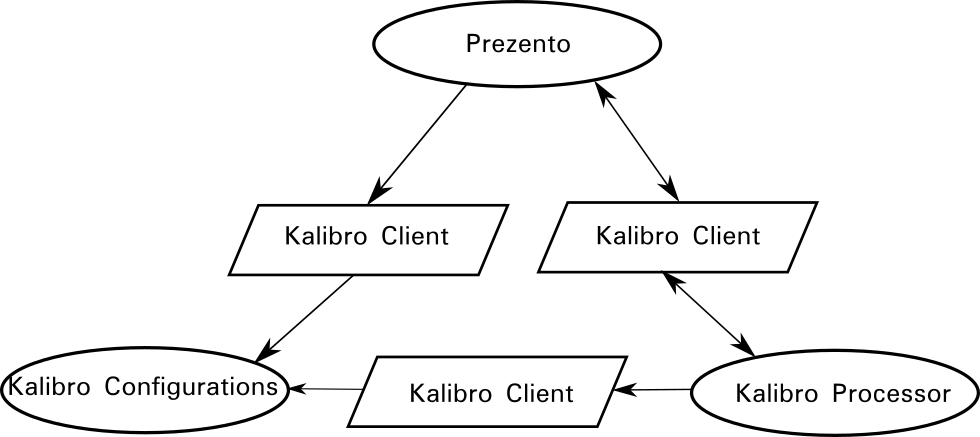
\includegraphics[width=.8\linewidth]{images/mezuro-architecturev3.png}
  \caption{Current Mezuro architecture.}
  \label{fig:architecture-2}
\end{figure}

The current Mezuro state is specified in Figure \ref{fig:architecture-2}.
Ellipses represents softwares involved and parallelograms the communication
interfaces between them. At Mezuro base we have Kalibro, segmented in three
smaller entities: Kalibro Processor, responsible for processing and evaluating
metrics; Kalibro Configurations, responsible for metrics definitions and
configurations; and Kalibro Client, responsible for interoperate communications
between these entities.  Prezento, the presentation layer, mainly communicates
with Kalibro Processor and Kalibro Configurations, via the Kalibro Client
interface.

\begin{figure}[hbt]
  \centering
    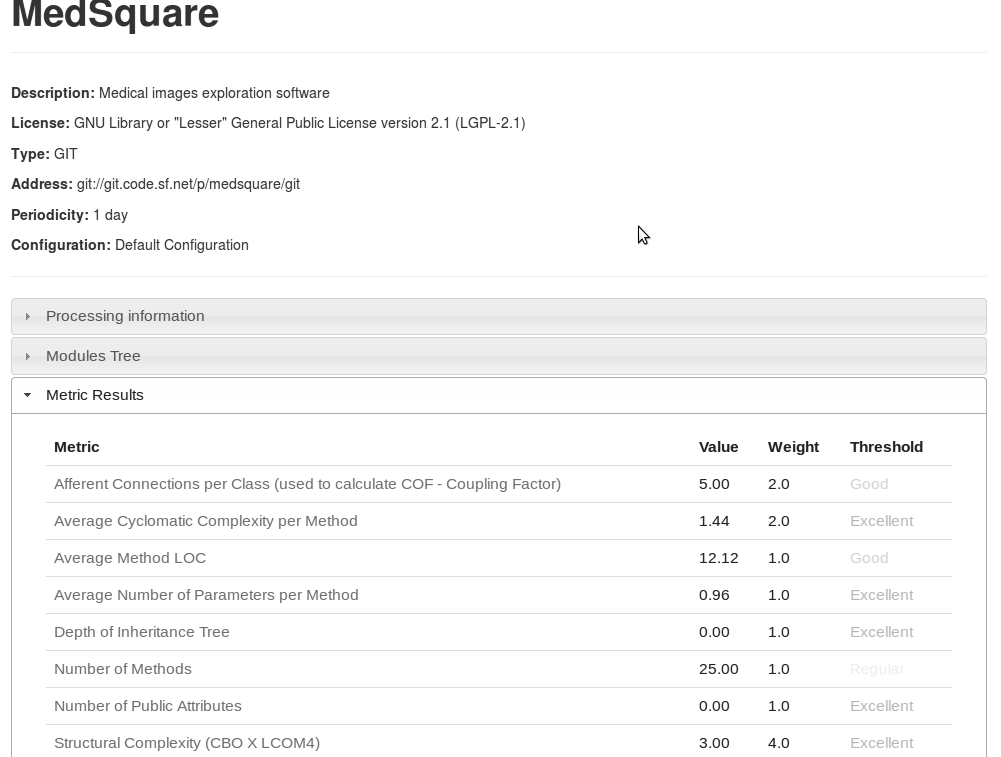
\includegraphics[width=.9\linewidth]{images/new-repository-results.png}
  \caption{Code analysis feature.}
  \label{fig:feature-1}
\end{figure}

Mezuro features can be divided in two groups:

\begin{itemize}
    \item Project (Figure \ref{fig:feature-1})

    \begin{itemize}
        \item Upload of source code via repositories (Git, Subversion, Bazaar etc) or via compressed file;
        \item Code process scheduling (1 day, 2 days, weekly, biweekly, and monthly);
        \item Definition of what metric configuration should be used for each file;
        \item Graphical analysis of each file via dotted plot with scores over time; % concordo que precisa mudar, mas acho que a sugestão dada ainda não soa tão bem.
        \item Public results that are accessible by the community.
    \end{itemize}
    \item Configuration
    \begin{itemize}
        \item Metric configuration cloning and creation;
        \item Statistics about most popular configurations in the community;
        \item Creation of qualitative ranges associated with values of metrics;
        \item Combination of native metrics to create composed and more complex analysis.
    \end{itemize}
\end{itemize}

Mezuro has also a strong learning aspect, in which participants are able to
observe other projects, or clone their configurations and definitions, to
learn with them.  This open mutual interaction is interesting to project
managers, software auditors and even an entire developer team. The final goal
is to create a community that see value in such methodologies and feel
comfortable to use them in their daily projects.

\section{Final remarks}

Mezuro architecture evolution is an answer to the lack of tracking and
standardization of source code analysis. It is a 100\% FOSS, highly
customizable, with support to many programming languages, providing a friendly
interface, for processing history and also with an extensible architecture
planned to easily embodying of new features by the FOSS community. Mezuro
source code is licensed under AGPLv3 and available at \url{github.com/mezuro},
as well as, it is in production at \url{mezuro.org}.

\bibliographystyle{splncs03}
\bibliography{mezuro}
\end{document}
